%----------------------------------------------------------
% PACKAGES AND THEMES
%----------------------------------------------------------
\documentclass[aspectratio=169,xcolor=dvipsnames,handout]{beamer}

\usetheme{Darmstadt}
\usecolortheme{seahorse}
\setbeamercovered{transparent}

\usepackage[hangul]{kotex}
\usepackage{hyperref}
\usepackage{graphicx, array, adjustbox, makecell}
\usepackage{booktabs, multicol, multirow}

% font조정
%\usepackage{fontspec}
%\setmainfont{Times New Roman}
%\setmainhangulfont{NanumGothic}

% 문자열 대체{노사관계론 전용}
\usepackage{newunicodechar}
\newunicodechar{•}{$\cdot$}
\newunicodechar{➔}{$\implies$}
\newunicodechar{∴}{$\therefore$}
\newunicodechar{∵}{$\because$}

%----------------------------------------------------------
% TITLE PAGE
%----------------------------------------------------------
\title{지역인재 채용정책은 대졸자 초임 격차를 줄일 수 있는가? 한국 대졸자 사례를 통한 인과적 추론}
\subtitle{Oh \& Lee, 2024, \textit{Economic Analysis and Policy}, 84, 208–229}
\author[Oh \& Lee]{오성재\inst{1} \and Hanol Lee\inst{2}}
\institute[CNU / SUFE]
{%
  \inst{1}
  %Department of Economics\\
  충남대학교\\
  %\vspace{0.2cm}
  \inst{2}
  %Research Institute of Economics and Management\\
  Southwestern University of Finance and Economics, China\\
  %\vspace{0.4cm}
  한국보건사회연구원
}
\date[Nov, 2024]{\today}

%----------------------------------------------------------
\begin{document}
%----------------------------------------------------------

\frame{\titlepage}

\begin{frame}{목차}
    \small
    \tableofcontents[hideallsubsections]
\end{frame}

\section{배경}
\begin{frame}
    \frametitle{지역간 격차 문제}
    \begin{itemize}[<+->]
        \item 수도권과 나머지 지역 간의 심각한 격차
        \begin{itemize}[<+->]
            \item 서울에 경제적, 사회적, 교육적 자원의 집중
            \item 서울의 GDP\@: 2022년 국가 전체의 22.7\% (통계청, 2022).
            \item 2020년 수도권과 비수도권 근로자 간 평균 임금 격차 9.8\% (Kang, 2023).
        \end{itemize}
        \item 심각한 교육 격차
        \begin{itemize}[<+->]
            \item 한국 상위 20개 대학 중 14개 대학이 서울에 위치 (QS 세계 대학 순위 2019)
            \item 비서울 대학 졸업생들의 노동 시장에서 불리한 위치.
        \end{itemize}
    \end{itemize}
\end{frame}

\begin{frame}
    \frametitle{지역인재 채용 의무화 정책}
    \begin{itemize}[<+->]
        \item 2007년 혁신도시법 시행
        \begin{itemize}[<+->]
            \item 수도권 내 공공기관과 기업의 집중을 분산시키고, 수도권 이외 지역의 지정된 혁신도시로 이전시키는 것을 목표.
        \end{itemize}
        \item 2013년 지역인재 채용 의무화 정책 도입
        \begin{itemize}[<+->]
            \item 공공부문이 지역인재를 일정 비율로 채용하도록 의무화하며, 경쟁력 있는 임금 및 보장된 임용기간을 제공 (Kim, 2019).
        \end{itemize}
        \item ``지역인재''
        \begin{itemize}[<+->]
            \item 서울, 인천, 경기를 제외한 지역에 위치한 대학의 졸업생(또는 졸업 예정자).
            \item 대학 캠퍼스가 위치한 지역이 유일한 기준이고, 해당지역에서만 지역인재로 인정.
        \end{itemize}
    \end{itemize}
\end{frame}

\begin{frame}[allowframebreaks]
    \frametitle{지역인재 채용 대상 공공부문}
    \begin{itemize}[<+->]
        \item 2020년까지 128개의 공기업 및 공공기관이 해당제도의 적용을 받음. 
        \item 지역인재 채용 비율은 2.8\%(2012)에서 14.2\%(2017)로 증가.
        \item 2022년까지 30\% 달성 목표 (대통령령).
        \item 채용대상 공공부문의 세 가지 변화
        \begin{enumerate}
            \item 기관의 지방이전 : 2013--2015년
            \item 지역간 통합 : 2016년 대구-경북, 2019년 충남-충북-대전-세종
            \item 신규 지정 : 2019년 충남, 충북, 대전, 세종
        \end{enumerate}
    \end{itemize}
    \begin{table}[ht]
        \centering
        \tiny
        \begin{tabular}{lccccccccc}
        \toprule
        & \multicolumn{8}{c}{\textbf{년도}} \\
        \cline{2-9} 
        \textbf{지역} & 2013 & 2014 & 2015 & 2016 & 2017 & 2018 & 2019 & 2020 \\
        \midrule
        부산     & 3 & 9  & 10 & 10 & 11 & 11 & 11 & 12 \\
        울산     & 0 & 6  & 6  & 6  & 6  & 6  & 7  & 7  \\
        경남 & 0 & 3  & 7  & 9  & 10 & 10 & 10 & 10 \\
        대구     & 2 & 7  & 9  & 16 & 16 & 16 & 16 & 16 \\
        경북  & 1 & 4  & 5  & 16 & 16 & 16 & 16 & 16 \\
        전북   & 1 & 2  & 4  & 5  & 6  & 6  & 6  & 6  \\
        광주   & 0 & 10 & 11 & 11 & 12 & 12 & 13 & 13 \\
        전남    & 0 & 10 & 11 & 11 & 12 & 12 & 13 & 13 \\
        대전    & 0 & 0  & 0  & 0  & 0  & 0  & 0  & 51 \\
        충북  & 3 & 6  & 7  & 7  & 8  & 9  & 10 & 51 \\
        충남 & 0 & 0  & 2  & 2  & 2  & 2  & 2  & 51 \\
        세종    & 1 & 14 & 18 & 18 & 19 & 19 & 19 & 51 \\
        강원   & 1 & 4  & 8  & 9  & 10 & 10 & 10 & 10 \\
        제주      & 0 & 0  & 1  & 1  & 1  & 3  & 3  & 3  \\
        \bottomrule
        \end{tabular}
        \caption{년도별 지역별 정책의 영향을 받는 기업의 수}
    \end{table}
\end{frame}

\section{주요 목표}
\begin{frame}
    \frametitle{연구 목표}
    \begin{itemize}[<+->]
        \item 비수도권 대학 졸업생과 수도권 대학 졸업생 간의 임금 격차 분석.
        \item 지역인재 채용 의무화 정책이 지역 임금 격차에 미치는 영향 조사.
    \end{itemize}
\end{frame}

\begin{frame}
    \frametitle{주요 발견}
    \begin{itemize}[<+->]
        \item 지역 간 초임 격차를 확인: 비수도권 대졸자는 수도권 대졸자 보다 10.9\% 낮은 초임을 받음.
        \item 정책은 비수도권과 수도권 소재 대졸자 간의 초임 격차를 효과적으로 좁힘.
        \item 인문계 전공 졸업생이 자연계 전공 졸업생보다 정책의 효과가 더 크게 나타남.
        \begin{itemize}[<+->]
            \item 이는 이전된 공공부문 일자리 특성 때문일 가능성 있음.
        \end{itemize}
        \item 정책은 비수도권 대학들이 교육의 질을 향상시키도록 유도하며, 초임 격차 감소에 기여함.
    \end{itemize}
\end{frame}

\begin{frame}
    \frametitle{이 글의 기여}
    \begin{enumerate}[<+->]
        \item 미시자료로 해당 정책의 노동 시장 성과에 미치는 영향을 측정한 첫 번째 연구.
        \item 대학 유형별로 신규 대졸자의 초임 격차 추정.
        \begin{itemize}[<+->]
            \item 기존에 축적된 경력 및 경험으로 인한 편향을 완화.
            \item 가장 영향을 받은 집단에 초점을 맞춤.
        \end{itemize}
        \item 정책 기제의 근본적인 작동 방식을 밝혀냄.
        \begin{itemize}[<+->]
            \item 정책은 비수도권 대학들이 교육의 질을 향상시키도록 유도함.
        \end{itemize}
    \end{enumerate}
\end{frame}

\section{자료와 모형}%

\begin{frame}
    \frametitle{자료}
    \begin{itemize}[<+->]
        \item 자료 출처: 대졸자 직업 이동 경로 조사 (GOMS) 2010--2019.
        \begin{itemize}
            \item 반복적인 횡단면 자료.
        \end{itemize}
        \item 조사 응답자는 대학 졸업 후 12--18개월 이내에 조사를 완료.
        \item 목표집단 : 4년제 대학 졸업 후 취업한 근로자.
        \begin{itemize}
            \item 제외된 대상 : 의예계열 졸업생, 편입생, 2009년 이전 졸업생, 해외 근무자, 병역 미이행자, 35세 이상.
        \end{itemize}
    \end{itemize}
\end{frame}

\begin{frame}[allowframebreaks]
    \frametitle{모형}
    \begin{enumerate}[<+->]
        \item 수도권과 비수도권 대졸자의 임금 격차를 분석.
        \begin{equation}
        \ln{(\text{wage})}_{i,j,p,t} = \alpha + \beta_1 \text{NonSeoul}_j + X_{i,t} \gamma + \tau_t + \epsilon_{i,j,p,t}
        \end{equation}
        \begin{itemize}[<+->]
            \item $\ln{(\text{wage})}_{i,j,p,t}$: t년도에 p지역에 위치한 j대학교를 졸업한 개인 i의 월급 로그.
            \item $\text{NonSeoul}_j$: 대학 j가 서울 외 지역에 위치하는지 여부를 나타내는 더미 변수.
            \item $X_{i,t}$: 통제 변수로 다음의 정보를 포함. 나이, 나이의 제곱, 근무 경력, 근무 경력의 제곱, 성별, 전공, 본교 캠퍼스를 다녔는지 여부, 응답자의 GPA의 백분위 범주, 그리고 특목고 졸업여부. 
        \end{itemize}
    \framebreak%
        \item 유형별 지방대학과 수도권 대학 간의 임금 격차를 조사.
        \begin{equation}
            \ln{(\text{wage})}_{i,j,p,t} = \alpha + \beta_8 \text{NonSMA}_j + X_{i,t} \gamma + \theta_p + \tau_t + \epsilon_{i,j,p,t}
        \end{equation}
        \begin{equation}
            \ln{\text{wage}}_{i,j,p,t} = \alpha + \beta_9 \text{KNU9}_j + \beta_{10} \text{PubUj}_j + \beta_{11} \text{PriUj}_j + X_{i,t} \gamma + \theta_p + \tau_t + \epsilon_{i,j,p,t}
        \end{equation}
        \begin{itemize}[<+->]
            \item 비교 집단: 서울 소재 대학을 순위 기준으로 두 가지로 범주화 : 1–20위와 21–50위.
            \item 지방거점국립대(지거국) ($\text{KNU9}_j$), 지방 국공립대 ($\text{PubUj}_j$), 지방사립대 ($\text{PriUj}_j$) : 서울 소재 대학에 비해 각 유형의 비수도권 대학의 임금 격차를 추정.
        \end{itemize}
    \framebreak%
        \item 이중차분법을 통해 수도권 비수도권 대졸자의 임금 격차에 대한 정책의 영향을 추정.% 
            \begin{align}
                \ln{\text{wage}}_{i,j,p,t} &= \alpha + \delta_1 D_{p,t} \text{nonSMA}_j + \beta_8 \text{nonSMA}_j + D_{p,t} \\ \nonumber
                    &\quad + X_{i,t} \gamma + \theta_p + \tau_t + \epsilon_{i,j,p,t} \\
                \ln{\text{wage}}_{i,j,p,t} &= \alpha + \delta_2 D_{p,t} \text{KNU9}_j + \delta_3 D_{p,t} \text{PubUj} 
                    + \delta_4 D_{p,t} \text{PriUj} + \beta_9 \text{KNU9}_j \\
                    &\quad + X_{i,t} \gamma + \theta_p + \tau_t + \epsilon_{i,j,p,t} \nonumber
            \end{align}
            \begin{itemize}[<+->]
                \item 통제 집단: 서울 소재 대학을 순위 기준으로 두 가지로 범주화 : 1–20 위와 21–50 위.
                \item $D_{p,t}$: t년에 p지역 대졸자가 지원 가능한 정책의 영향을 받는 공기업의 수.
            \end{itemize}
    \end{enumerate}
\end{frame}

\begin{frame}
    \frametitle{기초통계량}
    \begin{itemize}[<+->]
        \item 성과 변수는 2010년 원화로 측정된 월급의 로그값으로 평균 5.2, 이는 2010년 가격 기준으로 197만 원.
    \end{itemize}
    \begin{table}[ht]
        \tiny
        \centering
        \begin{tabular}{lcccc}
        \toprule
        \textbf{변수} & \textbf{평균값} & \textbf{표준분산} & \textbf{최솟값} & \textbf{최댓값} \\
        \midrule
        로그값 (월급, 2010 원화) & 5.188 & 0.453 & 3.117 & 6.244 \\
        $D_{p,t}$ & 3.816 & 5.243 & 0 & 19 \\
        지방대졸 & 0.750 & 0.433 & 0 & 1 \\
        지거국졸 & 0.172 & 0.377 & 0 & 1 \\
        지방국공립졸 & 0.108 & 0.310 & 0 & 1 \\
        지방사립대졸 & 0.470 & 0.499 & 0 & 1 \\
        \bottomrule
        \end{tabular}
    \end{table}
\end{frame}

\section{주요 결론}%
\begin{frame}
    \frametitle{지역간 초임 격차}
    \begin{table}[ht]
        \centering
        \tiny
        \begin{tabular}{lc}
        \toprule
        & \textbf{(1)} \\
        \midrule
        비수도권                    & -0.109***    \\
                                     & (0.007)      \\
        \midrule
        관측치                 & 79,899       \\
        $R^2$                    & 0.156        \\
        통제변수                     & 예          \\
        직장소재지 고정효과 & 예          \\
        졸업년도 고정효과 & 예          \\
        조사년도 고정효과 & 예          \\
        \bottomrule
        \multicolumn{2}{p{6cm}}{\tiny\textit{주} : 종속 변수는 실질월급의 로그값. 강건한 표준 오차는 괄호 안에 표시됨. ***는 1\% 수준 , *는 5\% 수준, 는 10\% 수준에서 통계적 유의성을 각각 나타냄.} \\
        \end{tabular}
    \end{table}
\end{frame}

\begin{frame}
    \frametitle{수도권-비수도권 지역간 초임격차}
    \begin{table}[ht]
        \centering
        \tiny
        \begin{tabular}{lcccc}
        \toprule
                                                   & \textbf{(1)} & \textbf{(2)} & \textbf{(3)} & \textbf{(4)} \\
        \midrule
         수도권 소재 기준대학의 순위 & 1--20     & 21--50    & 1--20     & 21--50    \\
        \midrule
        지방대학                       & -0.160*** & -0.102*** &           &           \\
                                                   & (0.009)   & (0.010)   &           &           \\
        지거국                                       &           &           & -0.117*** & -0.058*** \\
                                                   &           &           & (0.011)   & (0.012)   \\
        지방국공립대                &           &           & -0.149*** & -0.092*** \\
                                                   &           &           & (0.010)   & (0.011)   \\
        지방사립대               &           &           & -0.178*** & -0.119*** \\
                                                   &           &           & (0.009)   & (0.010)   \\
        \midrule                                    
        관측치                               & 57,909    & 49,743    & 57,909    & 49,743    \\
        $R^2$                                  & 0.167     & 0.153     & 0.167     & 0.153     \\
        통제변수                                   & 예       & 예       & 예       & 예       \\
        각종 고정효과                                        & 예       & 예       & 예       & 예       \\
        \bottomrule
        \multicolumn{5}{p{8cm}}{\tiny\textit{주} : 종속 변수는 실질월급의 로그값. 강건한 표준 오차는 괄호 안에 표시됨. ***는 1\% 수준 , *는 5\% 수준, 는 10\% 수준에서 통계적 유의성을 각각 나타냄.} \\
        \end{tabular}
    \end{table}
\end{frame}

\begin{frame}
    \frametitle{정책효과}
    \begin{table}[ht]
        \tiny
        \centering
        \begin{tabular}{lcc}
        \toprule
        & \textbf{(1)} & \textbf{(2)} \\
        \midrule
        수도권 소재 기준대학의 순위 & 1--20     & 21--50  \\
        \midrule                                                                                  
        지방대학 $\times D_{pt}$      & 0.003***  & 0.002**   \\
                                                  & (0.001)   & (0.001)   \\
        지방대학                      & -0.172*** & -0.110*** \\
                                                  & (0.009)   & (0.010)   \\
        \midrule                                                          
        관측치                              & 57,746    & 49,580    \\
        $R^2$                                 & 0.165     & 0.151     \\
        통제변수                                  & 예       & 예       \\
        각종 고정효과                                       & 예       & 예       \\
        \bottomrule
        \multicolumn{3}{p{6cm}}{\tiny\textit{주} : 종속 변수는 실질월급의 로그값. 강건한 표준 오차는 괄호 안에 표시됨. ***는 1\% 수준 , *는 5\% 수준, 는 10\% 수준에서 통계적 유의성을 각각 나타냄.} \\
        \end{tabular}
    \end{table}
\end{frame}

\begin{frame}
    \frametitle{비수도권 대학의 유형별 정책효과}
    \begin{table}[ht]
        \tiny
        \centering
        \begin{tabular}{lcc}
        \toprule
        \midrule
        수도권 소재 기준대학의 순위    & 1--20     & 21--50    \\
        \midrule                                                             
        지거국 $\times D_{pt}$                         & 0.003***  & 0.003*    \\
                                                     & (0.001)   & (0.001)   \\
        지방국공립대 $\times D_{pt}$  & 0.003***  & 0.003**   \\
                                                     & (0.001)   & (0.001)   \\
        지방사립대 $\times D_{pt}$ & 0.002***  & 0.001**   \\
                                                     & (0.001)   & (0.001)   \\
        지거국                                         & -0.134*** & -0.071*** \\
                                                     & (0.014)   & (0.014)   \\
        지방국공립대                  & -0.164*** & -0.104*** \\
                                                     & (0.012)   & (0.013)   \\
        지방사립대                 & -0.185*** & -0.124*** \\
                                                     & (0.009)   & (0.010)   \\
        \midrule                                                             
        관측치                                 & 57,909    & 49,743    \\
        $R^2$                                    & 0.169     & 0.125     \\
        통제변수                                     & 예       & 예       \\
        각종 고정효과                                          & 예       & 예       \\
        \bottomrule
        \end{tabular}
    \end{table}
\end{frame}

\begin{frame}
    \frametitle{대졸자 전공별 정책효과}
    \begin{table}[ht]
        \tiny
        \centering
        \begin{tabular}{lcccccc}
        \toprule
        \textbf{전공} & \multicolumn{2}{c}{\textbf{인문계열}}& \multicolumn{2}{c}{\textbf{자연계열}} \\
        \midrule                                                                                  
        수도권 소재 기준대학의 순위    & 1--20     & 21--50    & 1--20     & 21--50    \\
        \midrule                                                          
        지거국 $\times D_{pt}$                         & 0.004***  & 0.003*    & 0.004***  & 0.003**** \\
                                                     & (0.002)   & (0.002)   & (0.001)   & (0.001)   \\
        지방국공립대 $\times D_{pt}$  & 0.005***  & 0.004**   & 0.002*    & 0.002     \\
                                                     & (0.002)   & (0.002)   & (0.001)   & (0.001)   \\
        지방사립대 $\times D_{pt}$ & 0.003***  & 0.002**   & 0.002**   & 0.002**   \\
                                                     & (0.001)   & (0.001)   & (0.001)   & (0.001)   \\
        지거국                                         & -0.168*** & -0.050*** & -0.119*** & -0.111*** \\
                                                     & (0.013)   & (0.016)   & (0.012)   & (0.014)   \\
        지방국공립대                  & -0.199*** & -0.084*** & -0.149*** & -0.141*** \\
                                                     & (0.015)   & (0.018)   & (0.012)   & (0.014)   \\
        지방사립대                 & -0.238*** & -0.124*** & -0.155*** & -0.149*** \\
                                                     & (0.009)   & (0.013)   & (0.010)   & (0.012)   \\
        \midrule                                                          
        관측치                                 & 24,271    & 19,809    & 28,412    & 25,034    \\
        $R^2$                                    & 0.169     & 0.125     & 0.169     & 0.125     \\
        통제변수                                     & 예       & 예       & 예       & 예       \\
        각종 고정효과                                          & 예       & 예       & 예       & 예       \\
        \bottomrule
        \end{tabular}
    \end{table}
\end{frame}

\begin{frame}
    \frametitle{공통추세가정의 검증결과}
    \centering
    \begin{figure}
        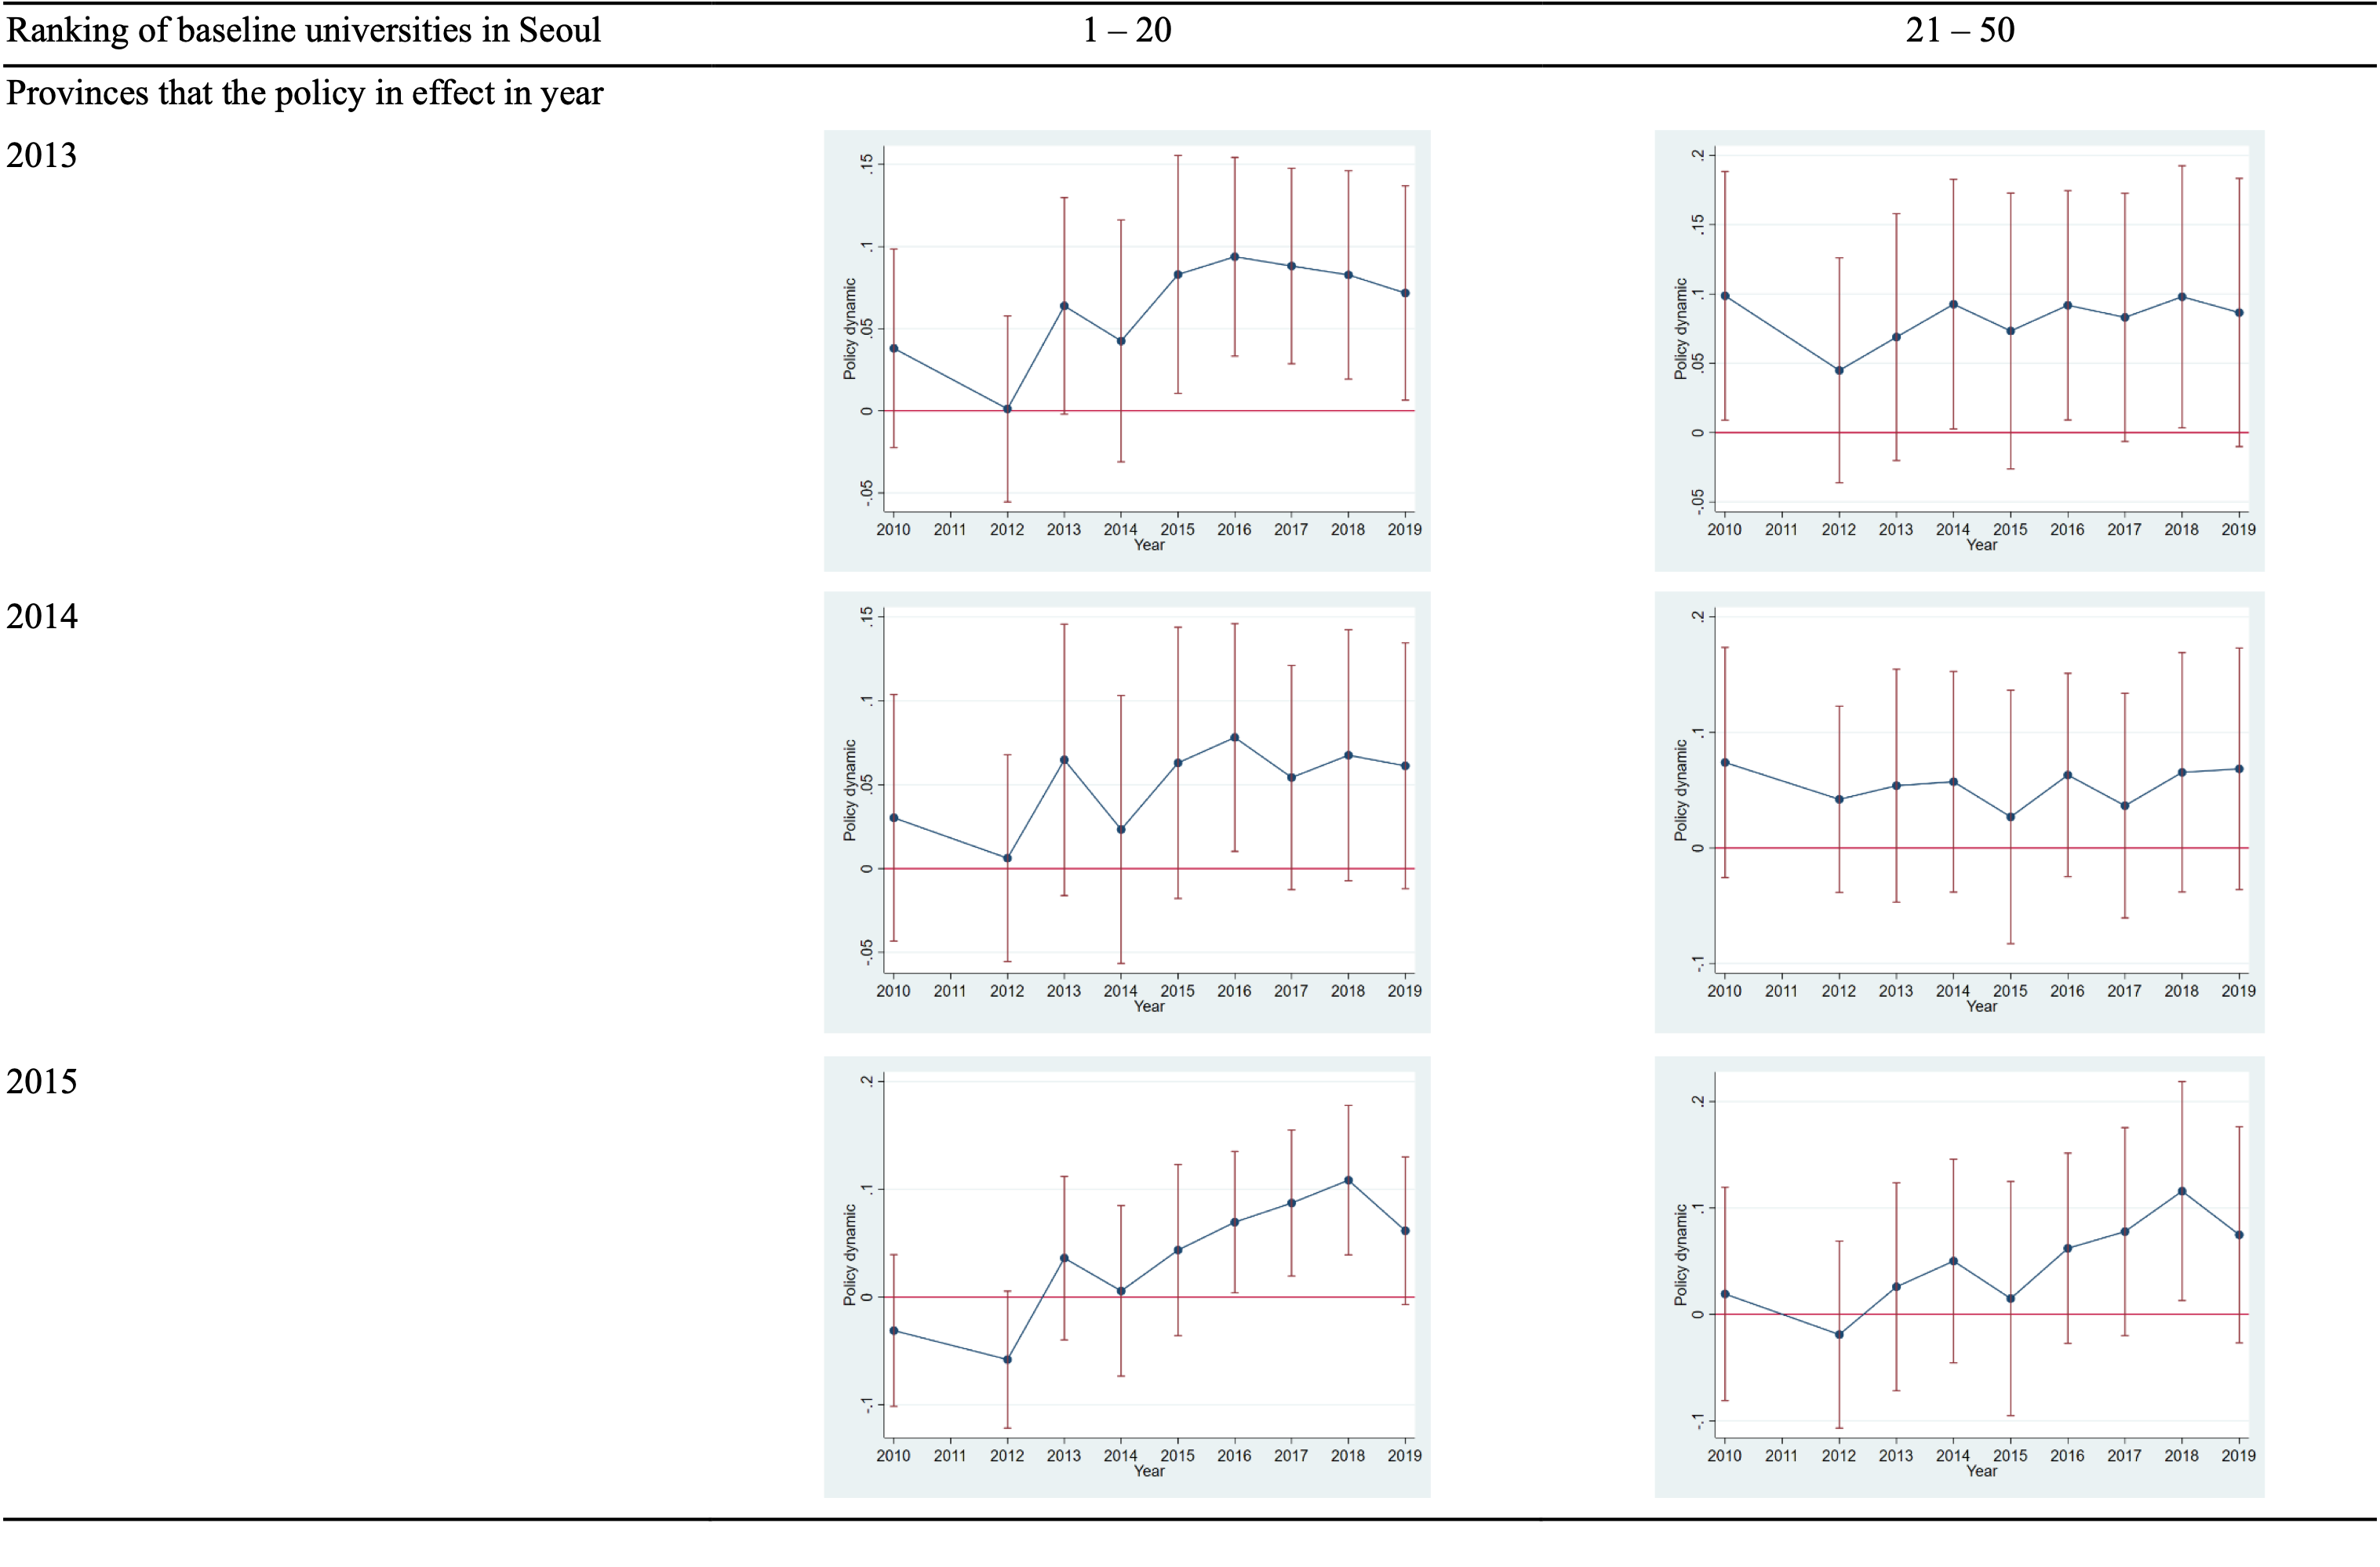
\includegraphics[width=.7\textwidth]{pic/pttest.png}
    \end{figure}
\end{frame}


\section{정책 기제}%
\begin{frame}
    \frametitle{정책 기제}
    두 가지 가능한 정책 기제:
    \begin{enumerate}[<+->]
        \item 대입에서 지원자의 행동 변화
        \begin{itemize}
            \item 서울에서 비수도권 대학으로의 이동 가능성
            \item 이는 비수도권 대학의 더 높은 질의 신입생을 유도할 수 있음
            \item 연구 설계는 이 효과를 완화함:
            \begin{itemize}
            \item 응답자의 대부분은 2013년 이전에 대학에 입학함.
            \item 인재 분포 변화로 인한 정책 효과는 우리 연구에서 배제됨.
            \end{itemize}
        \end{itemize}
        \item 비수도권 대학 교육의 질 향상
        \begin{itemize}
            \item 정책은 교육 질 향상을 유도함
            \item 취업 교육에 집중
            \item 이는 졸업생들의 더 나은 노동 시장 성과로 이어짐
        \end{itemize}
    \end{enumerate}
\end{frame}

\begin{frame}[allowframebreaks]
\frametitle{정책기제 가설의 검증}
    \begin{table}
        \tiny
        \centering
        \begin{tabular}{lcc}
        \toprule
        & (1) & (2) \\
        \midrule
        \textbf{종속변수} & \multicolumn{2}{p{3cm}}{\textbf{중앙일보 대학순위 2010--2019, 순위값에 -1을 곱함}} \\
        \midrule
        수도권 소재 기준대학의 순위 & \multicolumn{2}{c}{1--20} \\
        \midrule
        지거국 $\times$ Dpt & 0.239***   & 0.167***   \\
                        & (0.115)    & (0.100)    \\
        지거국              & -13.359*** & -14.744*** \\
                        & (1.070)    & (1.173)    \\
        \midrule
        관측치      & 118        & 118        \\
        $R^2$         & 0.647      & 0.785      \\
        통제변수          & 아니오         & 예        \\
        년도 고정효과           & 예        & 예        \\
        \bottomrule
        \multicolumn{3}{p{6cm}}{\tiny\textit{주} : 종속 변수는 대학의 순위. 통제 변수에는 교수진 수, 학생 1인당 장학금, 현장실습 참여학생 수, 해외대학교류 참여학생 수가 포함됨. 강건한 표준 오차는 괄호 안에 표시됨. ***는 1\% 수준 , *는 5\% 수준, 는 10\% 수준에서 통계적 유의성을 각각 나타냄.} \\
        \end{tabular}
    \end{table}
    \framebreak%
    \begin{table}
        \tiny
        \centering
        \begin{tabular}{lcc}
        \toprule
        & (1) & (2) \\
        \midrule
        \textbf{종속변수} & \multicolumn{2}{c}{\textbf{대학수준의 연간 학점 (0--100)}} \\
        \midrule
        수도권 소재 기준대학의 순위 & \multicolumn{2}{c}{1--20} \\
        \midrule
        지방대학 $\times D_{pt}$          & 0.065*** & 0.081*** \\
                                                & (0.025)  & (0.023)  \\
        지방대학                      & 1.207*   & -0.029   \\
                                                & (0.674)  & (0.828)  \\
        \midrule
        관측치                              & 1,678    & 1,678    \\
        $R^2$                                 & 0.037    & 0.064    \\
        통제변수                                  & 아니오       & 예      \\
        년도 고정효과                                   & 예      & 예      \\
        \bottomrule
        \multicolumn{3}{p{6cm}}{\tiny\textit{주} : 종속 변수는 대학 수준의 연간학점. 통제 변수에는 교수진 수, 등록된 학생당 장학금 수, 현장 실습 참여학생 수, 해외 대학 교류참여학생 수가 포함됨. 강건한 표준 오차는 괄호 안에 표시됨. ***는 1\% 수준 , *는 5\% 수준, 는 10\% 수준에서 통계적 유의성을 각각 나타냄.} \\
        \end{tabular}
    \end{table}
\end{frame}

\section{맺음말}%
\begin{frame}
    \frametitle{결론}
    \begin{itemize}[<+->]
        \item 지역인재 채용 의무화 정책은 지역간 초임 격차를 줄이는 데 기여.
        \item 비수도권 대학의 교육 질 향상.
        \item 정책은 지역간 균형발전을 촉진하는데 긍정적 효과를 야기.
        \item 공공부문에 집중
        \begin{itemize}
            \item 시뮬레이션 연구에 따르면, 민간의 대기업의 이전이 큰 영향을 미치는 것으로 나타남.(Jun, 2007).
        \end{itemize}
        \item 인재 채용의 지리적 제약.
        \begin{itemize}
            \item 인재 채용의 지리적 범위를 확장하여, 다른 지역의 지원자와 채용을 허용하면 정책의 효과성을 높일 수 있음.
        \end{itemize}
    \end{itemize}
\end{frame}

\begin{frame}
    \centering
    \huge
    감사합니다.
\end{frame}


%------------------------------------------------
\end{document}
%------------------------------------------------
